\documentclass[12pt,a4paper,oneside]{article}
\usepackage[spanish,english]{babel}
\selectlanguage{spanish}
\usepackage[T1]{fontenc}
\usepackage{times}
\usepackage[utf8]{inputenc}
\usepackage{amsmath}
\usepackage{graphicx}
\usepackage{multicol}
\usepackage{longtable}
\usepackage[refpages]{gloss}
\usepackage{float}
\usepackage{anysize}
\usepackage{bigstrut}
\usepackage{appendix}
\usepackage{lscape} 
\usepackage{pdflscape}
\usepackage{multirow}
\usepackage{listings}
\usepackage{color}
\usepackage{setspace}
\usepackage{enumerate} 
\usepackage{ragged2e}
\usepackage[utf8]{inputenc}
\usepackage{comment}
\usepackage{pslatex}
\usepackage{apacite} 
\usepackage{caption}
\usepackage{setspace}
\usepackage{imakeidx}
\bibliographystyle{apacite}
\makeindex
\usepackage[spanish,es-tabla]{babel}
\begin{document}
\renewcommand{\BOthers}[1]{et al.\hbox{}}
\renewcommand\bibname{Bibliografía}

%----------------------------------------------------------------------------------------
%	CONFIGURACION
%----------------------------------------------------------------------------------------
\marginsize{2.0cm}{2.0cm}{2.0cm}{2.0cm}

%----------------------------------------------------------------------------------------
%	Carátula
%----------------------------------------------------------------------------------------
\begin{titlepage}
\begin{center}
 {\Large \bf UNIVERSIDAD CATÓLICA DE SANTA MARÍA}\\
  \vspace{8mm} 
  {\Large \bf Facultad de Ciencias e Ingenieria Fisicas y Formales}\\
  \vspace{8mm}
  {\Large \bf Escuela Profesional de Ingeniería de Sistemas}\\
 \begin{figure}[H]
    \centering
    
\includegraphics[width=7cm]{Logo/logo de la catolica.png}
\end{figure}
\title{} % titulo de tu tesis para latex
{\Large \bf }
\vspace{1cm}
{\bf MEJORA DEL PROCESO DE RESERVACIONES DE RUTAS TURÍSTICAS DE UNA HOTELERA MEDIANTE LA IMPLEMENTACIÓN DE UN CHATBOT}\\[1.0cm]
\begin{flushright}
{\bf AUTOR}\\[0.5cm]
{Huanca Paucar Renato Denilzón}\\[0.5cm] % nombres del autor o autores [1.0cm]
{Sanchez Coila Arnold Bryan}\\[1.0cm]

{\bf ASESOR(A)}\\[0.5 cm] 
{Dra. Castro Gutierrrez Eveling Gloria}\\[0.5 cm] % nombre del asesor
\end{flushright}
\vspace{1cm}
{Arequipa - Perú}\\[0.5cm]
{2022}
\end{center}
\end{titlepage}

\pagenumbering{roman}
%----------------------------------------------------------------------------------------
%	Resumen
%----------------------------------------------------------------------------------------
\selectlanguage{spanish}
\begin{abstract}
\addcontentsline{toc}{section}{Resumen}
    Actualmente los sistemas de información pueden brindar un gran apoyo en el proceso de la reserva turística en un entorno hotelero, sin embargo, solo teniendo dichos sistemas aun hace falta personal para que pueda atender dudas o inquietudes que sean muy específicas por parte de los usuarios. Los sistemas de información son las herramientas adecuadas para gestionar y brindar información a los turistas, ya sean nacionales o internacionales, y así satisfacer sus necesidades. El turismo siempre ha sido una de las fuentes de ingresos más importantes para un país o una ciudad, por eso es tan importante contar con una adecuada gestión turística en nuestra ciudad, pues se espera que sea la satisfacción de los turistas. El enfoque de este documento se basa en el aporte de una inteligencia artificial que se encargue del procesamiento del lenguaje natural para que este pueda interactuar con el usuario y lo apoye en todo el ciclo de realización de la reserva turística en el hotel.
\end{abstract}

\newpage

%----------------------------------------------------------------------------------------
%	Abstract
%----------------------------------------------------------------------------------------

\selectlanguage{english}
\begin{abstract}
\addcontentsline{toc}{section}{Abstract}
    Actualmente los sistemas de información pueden brindar un gran apoyo en el proceso de la reserva turística en un entorno hotelero, sin embargo, solo teniendo dichos sistemas aun hace falta personal para que pueda atender dudas o inquietudes que sean muy específicas por parte de los usuarios. Los sistemas de información son las herramientas adecuadas para gestionar y brindar información a los turistas, ya sean nacionales o internacionales, y así satisfacer sus necesidades. El turismo siempre ha sido una de las fuentes de ingresos más importantes para un país o una ciudad, por eso es tan importante contar con una adecuada gestión turística en nuestra ciudad, pues se espera que sea la satisfacción de los turistas. El enfoque de este documento se basa en el aporte de una inteligencia artificial que se encargue del procesamiento del lenguaje natural para que este pueda interactuar con el usuario y lo apoye en todo el ciclo de realización de la reserva turística en el hotel. 
\end{abstract}
\selectlanguage{spanish}

\newpage

%----------------------------------------------------------------------------------------
%	Introducción
%----------------------------------------------------------------------------------------

\subsubsection*{\centering Introducción}
\addcontentsline{toc}{section}{Introducción}
El gran volumen de archivos dificulta su gestión si no cuenta con la ayuda del software específico que nos ayude. Pero la colaboración entre ingenieros y arquitectos aún es más complicada. Todos trabajan con diferentes archivos e información y, a menudo, ambas partes los actualizan manualmente, lo que es una fuente de errores y una pérdida de tiempo significativa. Al planificar el desarrollo de un proyecto es necesario definir los objetivos, los recursos que se asignan, el marco temporal y una estrategia de actuación. Esta estrategia puede definirse basándose en distintas metodologías ya existentes donde se realizaron una tabla de comparación para ver que metodología se adapta mejor a nuestro proyecto, según las necesidades y bondades del equipo encargado del proyecto.
\newpage

%----------------------------------------------------------------------------------------
%Índice
%----------------------------------------------------------------------------------------

\tableofcontents
\newpage

%----------------------------------------------------------------------------------------
%Planteamiento del Problema
%----------------------------------------------------------------------------------------
\section{PLANTEAMIENTO DE LA INVESTIGACIÓN}
\subsection{Planteamiento del Problema}
Muchas veces el uso de las tecnologías en nuestras épocas no son siempre la primera opción, debido a que ocurre falta de información sobre cómo la tecnología nos puede ayudar en varios aspectos de una empresa u organización. Actualmente, las empresas hoteleras utilizan métodos de registros poco convencionales y estos pueden presentar problemas tanto logísticos como administrativos donde esto conlleva una mala inversión de tiempo para los empleados de la empresa que se encuentra en la ciudad de Arequipa.   
Según \cite{Por2017} Una típica libreta o memoria de recepción, puede causar molestias a los clientes que llegan y no encuentran su reserva registrada en el sistema. La recepción de una hotelera tiene que ser acogedora, donde se debe administrarse adecuadamente y debe poder recibir datos de todos los clientes, además de proporcionar la información ingresada para realizar una reserva. Administre con precisión la información de cambios o cancelaciones de reservas para brindar soluciones rápidas y específicas a estas solicitudes. En ella suelen existir confusiones por extravío o extravío de información que no se puede almacenar. También se debe considerar las fechas de llegada y salida del hotel, especialmente en temporada alta cuando hay aviso de cancelación, llegada/salida anticipada y cambio de habitación durante la estancia. Según (Piedra, V., 2016) el problema que nos da a conocer es cómo las empresas hoteleras que no están adaptadas a la tecnología pueden presentar problemas al momento de llamar y realizar una reservación ya que se usa métodos poco convencionales como las libretas donde se coloca los datos de un cliente y estas pueden presentar mala escritura por parte del empleado. El desarrollar un sistema para esta empresa puede exhibir grandes mejoras de alta escalabilidad, ya que puede brindar servicios desde pequeñas empresas con pocos usuarios, hasta empresas con diferentes ubicaciones.  
Por otro lado (	Solano, M. 2012) los problemas que nos muestra los autores más comunes que se presentan en la sección de reservas suelen ser el almacenamiento de información sobre la habitación, como el tipo de habitación que tiene características comunes que necesitamos saber, así como su ubicación real en la casa. La correcta gestión de las fechas de entrada y salida del hotel es también otro quebradero de cabeza, sobre todo en temporada alta cuando a menudo hay cancelaciones, llegadas y salidas anticipadas, cambios de habitación durante la estancia. Gestionar adecuadamente la información sobre cambios o cancelaciones de reservas, dando soluciones rápidas y específicas a estas solicitudes donde muchas veces surgen confusiones por interrupción o pérdida de información almacenada, más que en la típica libreta o en la memoria del personal de recepción, es más frustrante para los huéspedes que llegan al check-in que sus solicitudes no se han tenido en cuenta.

\subsection{Objetivos de la Investigación}
\subsubsection{General}
    Mejorar el Procesos de Reservaciones de Rutas Turísticas mediante el uso de un chatbot.
\subsubsection{Específicos}
    \begin{itemize}
      \item {Estudiar el problema del inadecuado uso de los recursos tecnológicos en el proceso de reservas de habitaciones hoteleras.}
      \item {Realizar un análisis, diseño y construcción del Sistema.}
      \item {Desarrollar un sistema Escalable para su implementación.}
      \item {Validar las pruebas de correcciones de errores, bug y vulnerabilidades.}
      \item {Implementar un chatbot para la satisfacción del usuario.}
    \end{itemize}
\subsection{Preguntas de Investigación}
    \begin{itemize}
        \item {¿Cómo mejorar el sistema de reservas turísticas para la empresa hotelera?}
        \item {¿En qué medida el uso de la tecnología escalable puede influir en la gestión de reserva de la empresa hotelera?}
        \item {¿Cómo optimizar el flujo de búsqueda para el usuario del sistema de reserva?}
        \item {¿Cómo mejorar el sistema reportes de reservas en la empresa hotelera?}
    \end{itemize}
\subsection{Línea y Sublínea de Investigación a la que corresponde el Problema}
    Sistema de Información y Bases de Datos 
    
    Tiene como objetivo el estudio de modelos, procedimientos, métodos, técnicas y herramientas para la gestión, el desarrollo y la implantación de sistemas de información.
\subsection{Palabras Clave}
    Optimización, Tecnología Escalable, Reservaciones Turísticas.
\subsection{Solución Propuesta}
\subsubsection{Justificación del Problema}
    El desarrollo de este trabajo tiene como objetivo potenciar la gestión de reservas de la empresa hotelera, a través de nuevas tendencias tecnológicas desarrolladas, permitiendo así sistematizar y agilizar la operación de reservas, una de las ventajas más importantes. El uso de estas aplicaciones combinadas puede crear, tenemos lo siguiente:
    
    \begin{itemize}
        \item {Incluir un proceso de reserva adicional al proceso tradicional, asegurando una fuente adicional de ingresos y un servicio más completo para estos clientes.}
        \item {Ofrece horarios flexibles para reservar en cualquier momento.}
        \item {Tiempo reducido en el proceso de reserva.}
    \end{itemize}

\subsubsection{Descripción de la Solución}

    Para la solución de este proyecto se plantea el desarrollo de un sistema de información orientado tanto al lado de marketing, realizando una página web para la empresa, como al sistema de reserva, dicho desarrollo se realizará utilizando tecnologías como JavaScript en ES6, HTML5 y CSS3 como lenguajes fundamentales, también se hará uso del framework React JS para el apoyo del apartado de Front-End, luego el uso Node JS para el apartado de Back-End así como MySQL como motor de base de datos. Para esto del motor de base de datos se necesita realizar los modelados, por ende se usará UML. También se emplearán APIs de apoyo como Formik, styled-component, etc para facilitar el desarrollo de funciones básicas dentro del sistema. 
    Para el apartado de Front-End se orientará el desarrollo a SSR (Side Server Rendering), esto para optimizar en la medida de lo posible el SEO (Search Engine Optimization) y así la página web tenga el mejor impacto en los buscadores web que sea posible.

\subsection{ESTADO DEL ARTE O ESTADO DE LA CUESTIÓN}

    Recientemente en los últimos años la investigación sobre el uso de la implementación de tecnología para las empresas resulta muy beneficiosa ya que se puede optimizar las actividades dentro una empresa. Para esto, en el siguiente estado técnico, se buscó una serie de artículos que contenían mucha información relacionada con el tema de investigación; pero hay poca o ninguna información sobre su aplicación en nuestro país o sobre estudios relacionados con este tema. Luego, se detallará el contexto relacionado con el tema de investigación en otros países, detallando la metodología, implementación y algunas recomendaciones que tienen en su proyecto de investigación.\\
    El paper desarrollado por \cite{Felipe2022} es la realización de un chatbot para la atender a los clientes de un área de servicio, en este caso se centra para el área hotelera con lo que quiera, para esto de utilizar un bot llamado IBM Watson donde este bot contiene tecnología de computación cognitiva y la inteligencia web mediante la computación de la nube. Para el desarrollo y aplicación del bot en una hotelera se le tuvo que entrenar los patrones tales como realizar un saludo al cliente, mostrar los horarios de atención, ubicación,  entre otros que nos complejos para el bot, ya que el mismo autor reconoce que no son perfectos ya que padece de desventajas principales tales como el entendimiento del contexto dentro de una conversación para poder interactuar con el cliente para tener una experiencia agradable o el que, al no tener suficiente entrenamiento no puedan reconocer errores comunes que cometen las personas al escribir por un canal digital.\\ El resultado que se obtuvo fue de 75 porciento de solicitudes respondidas, las cuales fueron las ubicaciones, los horarios del hotel, servicios que se realizan. Para el autor fue todo un logró integrar este bot porque los clientes tuvieron una experiencia con la tecnología de una hotelera. Tal como indica el autor del paper es implementar tecnología en un servicio hotelero sino en todas las áreas de servicio al cliente, el implementar un bot a nuestro proyecto es bastante interesante ya que mejora la experiencia del cliente con la hotelera, no se descarta la idea de implementar este bot con la tecnología que usa el autor del paper. 
    De acuerdo con los autores del paper nos habla de una implementación de un chatbot de IBM   llamado Watson, el cual permitirá crear un asistente virtual para los turistas de la ciudad de Jaén. Para el desarrollo de esta es usar CMS Wordpress y el uso de un plugin de IBM para la interacción con el bot. La metodología para el desarrollo de este proyecto es SCRUM que es una metodología ágil ya que permite llevar a cabo el análisis y diseño en cada ciclo, para esto se tuvieron que utilizar algunos lenguajes en conocimientos como el Nodejs, Angular.  Los autores como resultados tuvieron respuestas experimentales creadas por los propios autores donde ellos aplicaron machine learning para el entrenamiento. De acuerdo con lo mencionado, el uso de implementar un chatbot es bastante interesante para nuestro proyecto ya que se puede entrenar al bot watson para responder algunas preguntas clave para que interactúe con el usuario, pero el uso de la tecnología de Wordpress no va de acuerdo con nuestro proyecto ya que no es una tecnología escalable ya que esto no permite realizar algunas modificaciones al sistema.\cite{Muñoz2018}\\Los autores presentan como integrar el aprendizaje por refuerzo profundo para modelar a un chatbot esto con un refuerzo de recompensa futura, se simulan diálogos entre dos agentes virtuales y estos se evalúan por diversidad, longitud y evaluadores humanos para de esta forma demostrar que el algoritmo propuesto es capaz de generar respuestas interactivas y que pueda lograr una conversación sostenida, los modelos presentados en el artículo se tiene en cuenta para el desarrollo del chatbot planteado en nuestro documento. Por otra parte hablar sobre las tendencias que existe entre los destinos turísticos y las empresas turísticas que se consideran los hoteles, agencias de viaje, o las agencias en línea. Para esto los autores de este paper nos mencionan el uso de un chatbot para la atención de clientes. Para esto la implementación los autores nos habla de Kayak ya que es utilizado en las plataformas de facebook, messenger, en algunos blogs y en Slack. Los autores nos mencionan que el uso de este chatbot es mediante reglas, es decir, que está programado para obedecer a flujos de navegación bien definidos, que estos responden a ciertos comandos y palabras clave. Con respecto a la validación de este paper los autores nos mencionan que realizaron una encuesta con unos alumnos de la carrera de turismo de una universidad, para que interactúen con el chatbot, que da como resultado un chatbot con un desarrollo de alto nivel. El paper que elaboraron los autores es bastante importante hacia nuestro proyecto ya que la implementación del chatbot hacia un área de una empresa hotelera es muy interesante que se ve como optimizar o mejorar algunos apartados para la hotelera, se toma en cuenta el método de evaluación y los resultados obtenidos.\cite{Dias2020} \\
    Por otro parte los autores nos hablan de un chatbot que llamaron catbot el cual fue entrenado  con un sistema que también realizaron el cual está orientado para su uso por parte de la recepcionista del hotel, esto permitiría dar información para el entrenamiento del chatbot a su vez este chatbot estaría en directo entrenamiento con las necesidades y consultas del cliente, el tener un sistema para la recepcionista también es más optimo debido a la automatización de la recopilación de los datos para el entrenamiento, la metodología usada consta de 4 pasos los cuales son recopilación de requisitos, creación del diseño del sistema de información, la información del diseño del sistema y la evaluación de los resultados de evaluación, se considera una propuesta interesante el hecho de tener un sistema que esté apto para la recopilación de datos para posteriormente usarlos para poder usar estos datos en el entrenamiento de un chatbot personalizado para el sistema, por ende se tomara en consideración en la implementación nuestra propuestas.\cite{Levannoza2020} \\
    La importancia del uso de tecnologías basadas en AI, para esto los autores nos mencionan de una implementación de un chatbot llamado Smart Guidance para la interacción de los turistas el cual será llevado a un entorno de tecnología móvil. Para este desarrollo tuvieron que utilizar Android Studio, Firebase, Python, para esto se simula un chat con los usuarios en lenguaje natural, además proporciona una interacción bidireccional y es un único punto de contacto para todas las comunicaciones de los usuarios. Con respecto a la validación los autores del paper demostraron que el bot podía entender los significados y las solicitudes de los usuarios, donde se llevó a cabo un caso de uso en la ciudad de Jeddah, Arabia Saudita. Jeddah es la segunda ciudad más grande de Arabia Saudita. De Acuerdo con lo descrito, los autores de este paper nos mencionan la importancia de usar un bot dentro de un sistema de información o un desarrollo móvil para los usuarios, el uso de las tecnologías mencionadas para llevar a cabo son bastantes interesantes ya que usan lenguajes actuales y de fácil manejo en su entorno, se tomará en cuenta el desarrollo de su proyecto para nuestra propuesta de mejora para las empresas hoteleras en la ciudad de Arequipa.\cite{Alotaibi2020}
    Al ver terminado de realizar el estado del arte, el uso de tecnología escalable específicamente  en el desarrollo web, muestran que los autores usan este apartado para resolver varios de los problemas que presentan dentro de las empresas; podemos concluir que varios de los autores que presentan el uso de las tecnologías escalables que pueden ser utilizadas para el desarrollo del sistema de reserva hotelera en Arequipa ya que se demuestra que el desarrollo de sistemas escalables son muy beneficios para una empresa. 



%----------------------------------------------------------------------------------------
%Fundamentos Teóricos
%----------------------------------------------------------------------------------------
\section{Fundamentos Teóricos}
%\subsection{Estado del Arte}
   % Recientemente en los últimos años la investigación sobre el uso de la implementación de tecnología para las empresas resulta muy beneficiosa ya que se puede optimizar las actividades dentro una empresa. Para esto, en el siguiente estado técnico, se buscó una serie de artículos que contenían mucha información relacionada con el tema de investigación; pero hay poca o ninguna información sobre su aplicación en nuestro país o sobre estudios relacionados con este tema. Luego, se detallará el contexto relacionado con el tema de investigación en otros países, detallando la metodología, implementación y algunas recomendaciones que tienen en su proyecto de investigación.

  %Los autores presentan como integrar el aprendizaje por refuerzo profundo para modelar a un chatbot esto con un refuerzo de recompensa futura, se simulan diálogos entre dos agentes virtuales y estos se evalúan por diversidad, longitud y evaluadores humanos para de esta forma demostrar que el algoritmo propuesto es capaz de generar respuestas interactivas y que pueda lograr una conversación sostenida, los modelos presentados en el artículo se tiene en cuenta para el desarrollo del chatbot planteado en nuestro documento.
\subsection{Bases Teóricas de la Investigación}
\begin{itemize}
  \item Turismo\\
  Como parte del turismo tenemos a la Organización mundial del Turismo (OMT) “El turismo comprende las actividades que realizan las personas durante sus viajes y estancias en lugares distintos al de su residencia habitual por menos de un año y con fines de ocio, negocios, estudio, entre otros”
\item Información Turística \\
  Según el autor Exponemos la definición de Centeno, Doffourt y García (2011) “La información turística no es diferente de cualquier otra información. Solo se distingue por su utilidad en el entorno de la actividad turística. Así podemos considerar información turística tanto la información de la oferta turística de un destino y de sus precios como aquella que nos explica las tendencias de la demanda”.
  \item Machine Learning \\
  Es  parte de una rama de la inteligencia artificial y la informática que se enfoca en usar datos y algoritmos para imitar la forma en que aprenden los humanos, mejorando gradualmente su precisión.
  \item Chatbot \\
  Los chatbots son software o programas informáticos que simulan una conversación humana o "chat" a través de interacciones de texto o voz. Un aspecto importante de la implementación de un chatbot es la elección de un motor de procesamiento de lenguaje natural
  \item Inteligencia Artificial\\
  La inteligencia artificial es una rama amplia de la informática que se ocupa de construir máquinas inteligentes capaces de realizar tareas que normalmente requieren inteligencia humana.
  
\end{itemize}
%----------------------------------------------------------------------------------------
%Marco Metodológico
%----------------------------------------------------------------------------------------
\section{Aspecto Metodológicos}
\subsection{Alcance y Limitaciones}
El aporte de este proyecto a desarrollar es ayudar a las empresas hoteleras a contar con un sistema de escalabilidad, ya que les puede permitir agregar nuevos requerimientos al sistema tanto por el usuario como a los clientes, ya que si no se pudiera realizar este tipo de modificaciones se tendría que migrar a otro sistema o el mantenimiento pueda ser complejo, lo cual elevaría los costos para la empresa adquirir un nuevo sistema. 
\subsection{Tipo de Estudio}
\begin{itemize}
  \item Cuantitativo: Es un estudio cuantitativo donde se utilizará datos para poder medir la satisfacción del cliente.
  \item Experimental: Para el tipo de estudio de esta investigación es experimental, ya que se realizarán pruebas de la implementación.
  \end{itemize}
\subsection{Diseño}
El objetivo del diseño es desarrollar la interfaz es que tenga entre la funcionalidad y el contenido que guie al usuario en la interacción con la aplicación. El diseño de la interfaz define detalles como: la página de inicio, la página de bienvenida para el usuario, la página de login para el usuario, la página de login para el cliente. Para esta aplicación, se tiene que cumplir las seis etapas del diseño de una aplicación web.
Para el diseño de la arquitectura, Esta parte del diseño amarra al título del proyecto, los usuarios y las políticas de navegación. Es la forma en que el contenido se estructura y cómo la aplicación maneja la interacción con el usuario, los mapas de navegación. Existen distintas formas de las cuales elegimos dos opciones sobre la arquitectura: la de dos capas y la de tres capas.\\ Donde el cual se realizó una comparación teoría y aplicada donde se obtuvo como resultado la arquitectura de dos capas para nuestro proyecto de desarrollo.Como último paso para el diseño de los componentes, el Diseño y construcción de los programas que manejen los datos y generen las páginas que conforman la aplicación. 
\subsection{Universo (ámbitos) y muestra (informantes) (si se necesita)}
El universo comprende a todos los hoteles de que no cuenten con un sistema automatizado o que cuenten con un sistema poco o no escalable, de esta manera los datos tomados serán considerados para tener en cuenta las necesidades relacionadas con las reservas turísticas.Por parte de las muestras se tomará en cuenta a los hoteles que se encuentre en la ciudad de Arequipa para la obtención de los datos. 
\subsection{Técnicas e Instrumentos}
Es necesario basarse en unas definiciones relacionadas con el objeto de estudio que es la tecnología escalable. Para esto se definió la tecnología escalable mediante el uso de framework, en el ámbito del desarrollo web, es por ello que los puntos relativos al sistema de reservas se identificarán como conceptos, características, entre otras cosas relacionadas con ella; así como todo lo relacionado con el desarrollo del sistema web, como su funcionamiento, características de, lenguajes de programación, métodos de desarrollo, etc. Para del desarrollo del sistema se tomará en cuenta la arquitectura de 3 capas, esta arquitectura dada en el framework a trabajar nos ayudará en varios aspectos importantes del producto final, tales como la seguridad la escalabilidad y la optimización tanto por parte de los procesos como del SEO (Posicionamiento en buscadores). 
\subsection{Procesamiento de la Información y Análisis de Resultado}
Se pretende usar la metodología ágil; existen muchos métodos de desarrollo ágil, donde la mayoría trata de minimizar los riesgos desarrollando software en cortos lapsos de tiempo. El software desarrollado en una unidad de tiempo es llamado un sprint, el cual debe durar de una a cuatro semanas. Cada sprint del ciclo de vida incluye: planificación, análisis de requerimientos, diseño, codificación, revisión y documentación. Un sprint no debe agregar demasiada funcionalidad para justificar el lanzamiento del producto al mercado, pero la meta es tener un demo (sin errores) al final de cada sprint. Al final de cada sprint el equipo vuelve a evaluar las prioridades del proyecto. Muchos métodos similares al ágil fueron creados antes del 2000. Entre los más notables se encuentran: Scrum (1986), Crystal Clear (cristal transparente), programación extrema o XP (1996), desarrollo de software adaptativo, feature driven development, Método de desarrollo de sistemas dinámicos (1995). Kent Beck creó el método de Programación Extrema (usualmente conocida como XP) en 1996 como una forma de rescatar el proyecto del Sistema exhaustivo de compensaciones de Chrysler (C3). Mientras Chrysler cancelaba ese proyecto, el método fue refinado por Ron Jeffries.Ya con la definición más clara se optó por la metodología Scrum, La Metodología Scrum es un proceso de desarrollo de software iterativo y creciente utilizado, comúnmente, en entornos basados en el desarrollo ágil de software. Scrum es un framework de desarrollo ágil de software. El trabajo es estructurado en ciclos de trabajo llamados Sprints, iteraciones de trabajo con una duración típica de dos a cuatro semanas. Durante cada sprint, los equipos eligen de una lista de requerimientos de cliente priorizados, llamados historias de usuarios, para que las características que sean desarrolladas primero sean las de mayor valor para el cliente. Al final de cada sprint, se entrega un producto potencialmente lanzable / distribuible / comerciable. Scrum se caracteriza por ser un modelo que define un conjunto de prácticas y roles que puede tomarse como punto de partida para definir el proceso de desarrollo que se ejecutará durante un proyecto. Los roles principales en Scrum son el Scrum Master, el Product Owner, y el Equipo Scrum. Para el desarrollo de esta investigación se pretende usar la metodología Scrum, ya que es la que mejor se acopla a nuestro proyecto de investigación debido a que proporciona la adaptación, flexibilidad y rapidez para ajustar el proyecto a las circunstancias del entorno. A continuación, se describirán las fases de la ejecución de la metodología seleccionada.
\section{Cronograma}
Para el apartado del desarrollo se utilizará el Diagrama Gantt. Donde se mostrarán las actividades que se desarrollaron durante este proceso de desarrollo. 
\begin{figure}[H]
    \centering
    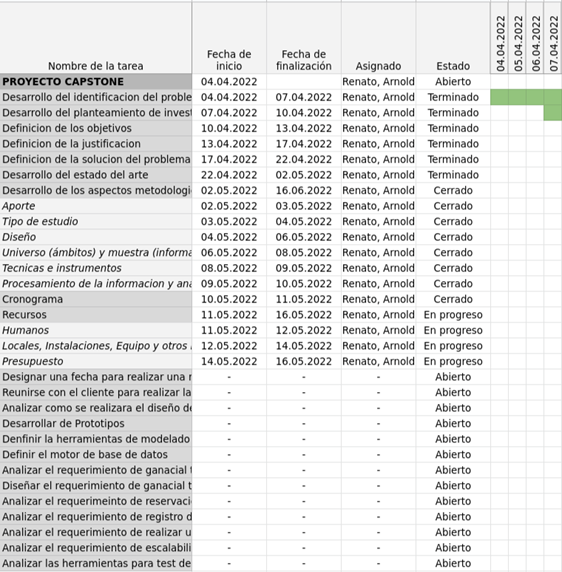
\includegraphics[width=15cm]{Recursos/d.PNG}
    \caption{Diagrama de Gantt del proyecto}
    \label{fig:projectGantt}
\end{figure}
\begin{figure}[H]
    \centering
    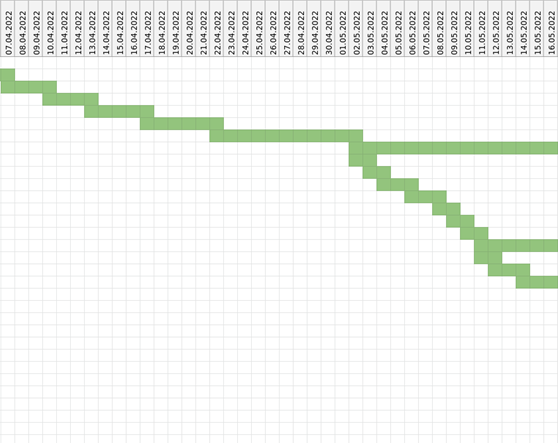
\includegraphics[width=15cm]{Recursos/e.PNG}
    \caption{Continuación del diagrama de Gantt del proyecto }
    \label{fig:projectGantt2}
\end{figure}
\section{Recursos}
Para el apartado del desarrollo se utilizará el Diagrama Gantt. Donde se mostrarán las actividades que se desarrollaron durante este proceso de desarrollo. 
\subsection{Humanos (Organización, Descripción de funciones, Personal)}
Los recursos humanos necesarios para el desarrollo e implementación de la solución (aplicativo web) son los que se muestran a continuación en la Tabla I.
 \begin{figure}[H]
    \centering
    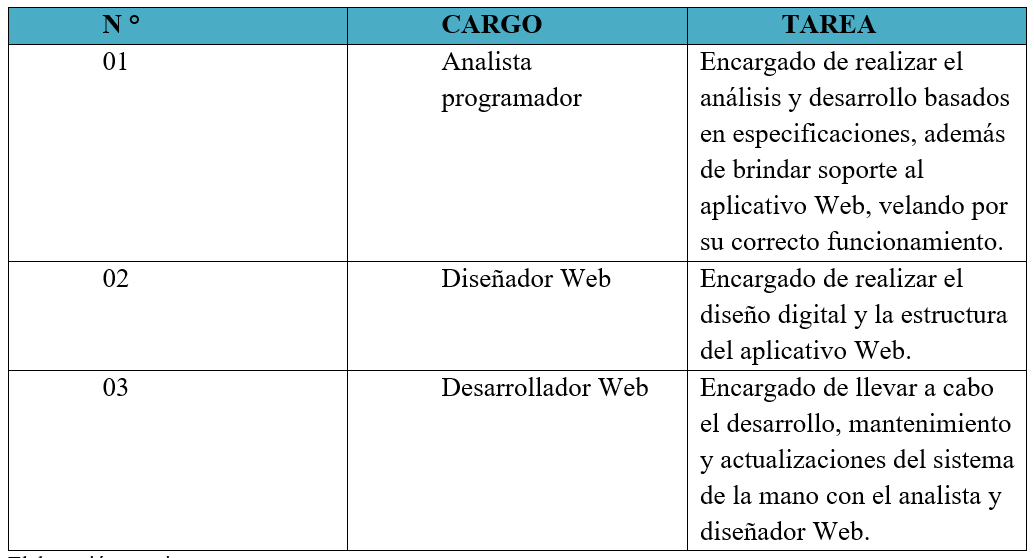
\includegraphics[width=15cm]{Recursos/a.PNG}
    \caption{Recursos Humanos necesarios para el desarrollo del proyecto}
    \label{fig:rrhhNeeded}
\end{figure}

\subsection{Locales, Instalaciones, Equipo y otros recursos}
La Tabla II muestra el software necesario que se utilizara para el desarrollo del sistema web.
\begin{figure}[H]
    \centering
    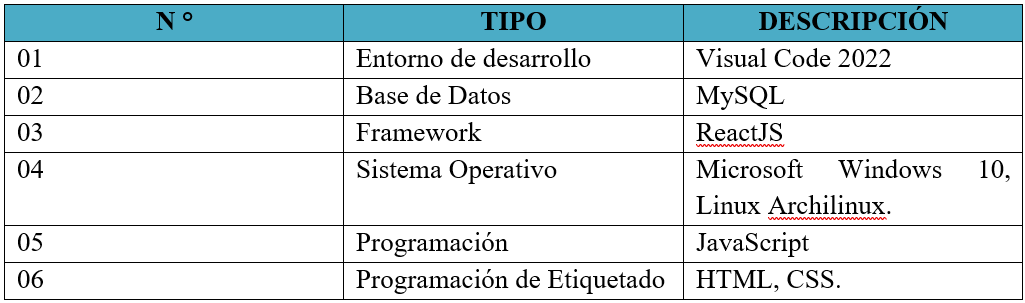
\includegraphics[width=15cm]{Recursos/b.PNG}
    \caption{Lista de Software necesario para el desarrollo del Proyecto}
    \label{fig:softwareNeeded}
\end{figure}
\subsection{Presupuesto}
Para este apartado se realizó un estimado del costo de producción del software donde se muestra en la Tabla III a continuación:
\begin{figure}[H]
    \centering
    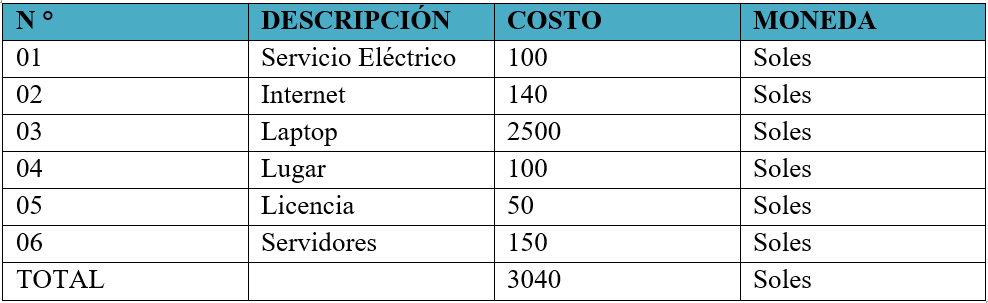
\includegraphics[width=15cm]{Recursos/c.PNG}
    \caption{ Lista de Presupuesto necesario para el desarrollo del Proyecto en Meses}
    \label{fig:budget}
\end{figure}
\newpage
\bibliography{sample}
\end{document}